\begin{figure*}[t!]
\vspace{-2mm}
  \begin{minipage}[t]{.31\linewidth}
    \centering
     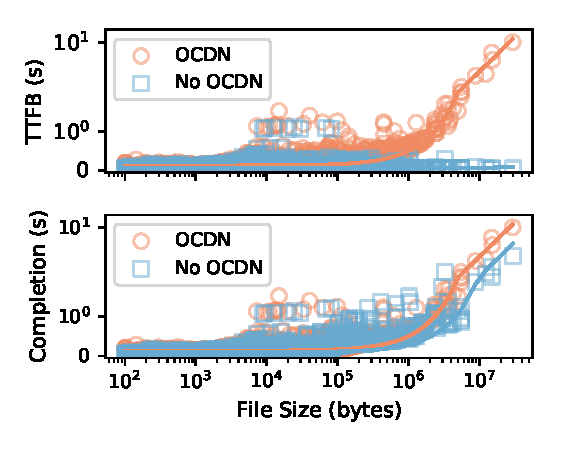
\includegraphics[trim={10 15 10 12},clip,width=\textwidth]{combined}
    \caption{Time to first byte and time to complete a request with and without \system{}.}
    \label{fig:completion}
  \end{minipage}
  \hfill
  \begin{minipage}[t]{.29\linewidth}
    \centering
    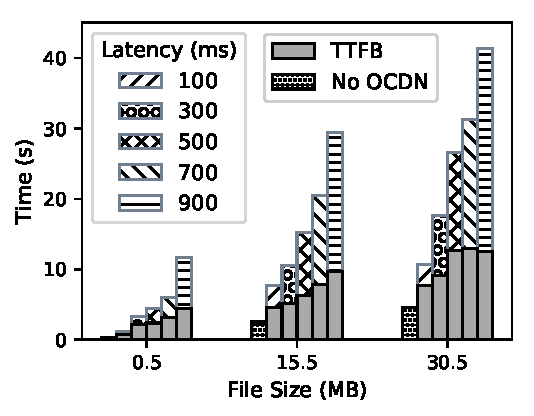
\includegraphics[trim={7 0 10 5},clip,width=\textwidth]{Latency_withoutzero_2}
    %\vspace{-10mm}
    \caption{Time to first byte and time to complete a request with varying the file size and latency; this latency 
corresponds to $\alpha$ in Figure \ref{fig:impl}.}
    \label{fig:latency}
  \end{minipage}
  \hfill
  \begin{minipage}[t]{.35\linewidth}
    \centering
    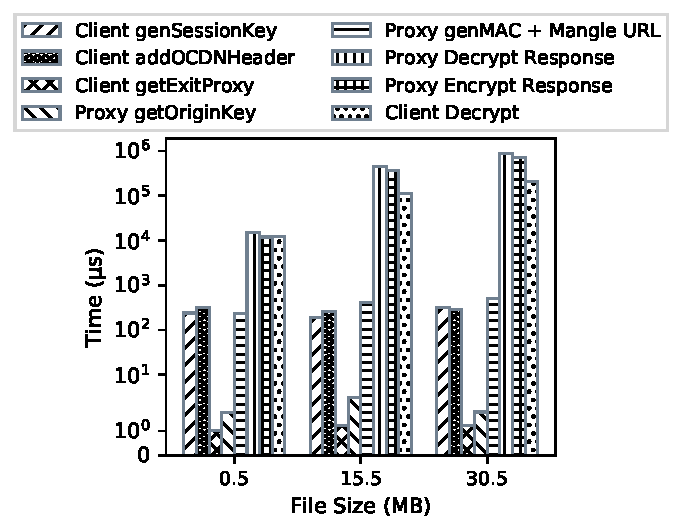
\includegraphics[trim={7 8 7 7},clip,width=\textwidth]{loggrouped_2}
\caption{Overhead of different operations performed by \system{}.}
\label{fig:overhead2}
  \end{minipage}
\end{figure*}


\section{Performance Analysis}
\label{sec:performance}
To evaluate how much overhead is caused by \system{} we measure the performance 
of \system{}.  In addition to understanding the latency and overhead produced by the 
system, we also discuss the scalability of the design and show how \system{} scales 
well with an increasing number of clients.

\subsection{\system{} Overhead}
For measuring performance characteristics of \system{}, we use the implementation 
described in Section \ref{sec:implementation}.  Figure \ref{fig:impl} shows 
how our measurements reflect \system{} (solid line) and a traditional CDN (dotted 
line).  

Figure \ref{fig:ttfb} shows the time to first byte (TTFB) for both \system{} and 
without \system{}.  We can see the the TTFB using \system{} grows linearly with 
file size, whereas without \system{} TTFB remains fairly constant.  Interestingly, 
we can see that there are some fixed time operations that \system{} performs, which 
is visible by looking at the smaller file sizes.

%\begin{figure}[t!]
%\centering
%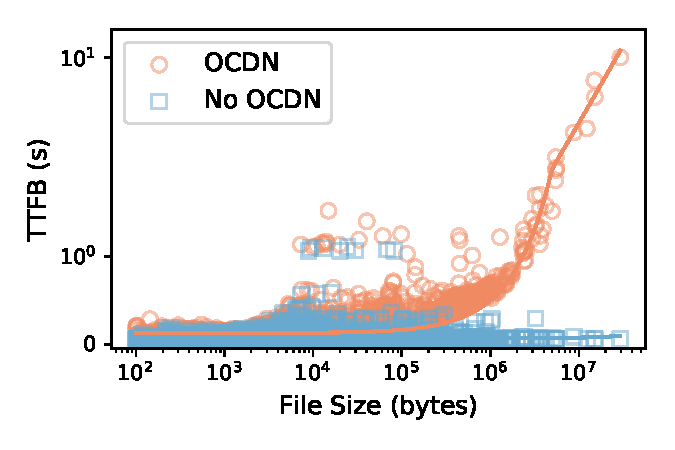
\includegraphics[width=.4\textwidth]{TTFB}
%\caption{Time to first byte measurements with and without \system{}.}
%\label{fig:ttfb}
%\end{figure}

In addition to measuring TTFB, we measured the time it took to complete a request (with and 
without \system{}); the results are shown in Figure \ref{fig:completion}.  Again, completion time 
grows linearly with file size, but for both \system{} and without \system{}; while both follow the 
same pattern, the time to complete requests is, as expected, longer using \system{} as it performs 
many cryptographic operations and proxies traffic between the client and the CDN.  

%\begin{figure}[t!]
%\centering
%\includegraphics[width=.4\textwidth]{completion}
%\caption{Time to complete a request with and without \system{}.}
%\label{fig:completion}
%\end{figure}

As described in Section \ref{sec:implementation}, our prototype included only a single client, but 
our design allows for a client to proxy her request through additional clients.  To simulate this, we 
add latency between the client and the exit proxy, and measure both the TTFB and time to complete a request 
when there are different values of latency, which represent different numbers of clients on the path between the 
original client and the exit proxy.  Figure \ref{fig:latency} shows the results for three different file sizes. The 
bottom portion of each bar in the graph shows the TTFB, and the top portion shows the additional time needed 
to complete the request.  As expected, the TTFB grows much slower as file size and latency increase; completion time 
grows more quickly than TTFB as the file size and latency increase.   

%\begin{figure}[t!]
%\centering
%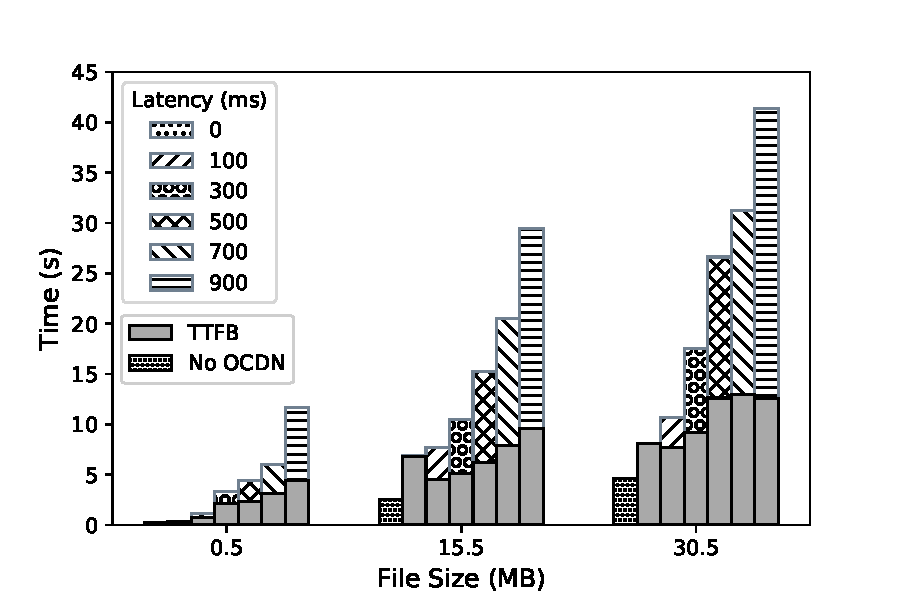
\includegraphics[width=.4\textwidth]{Latency_withzero}
%\caption{Time to first byte and time to complete a request with varying the file size and latency; this latency 
%correspondes to $\alpha$ in Figure \ref{fig:impl}.}
%\label{fig:latency}
%\end{figure}

Finally, we measure the performance overhead of the individual operations used in
\system{}; figure \ref{fig:overhead2} shows
the overhead of different components of the system for three different file sizes.  We can see that some of the fixed cost/time 
operations include the client locally looking up the correct exit proxy to use for a given URL and the exit proxy generating the 
HMAC$_{k}$(URL).  The operations that have the most overhead and continue to grow with the size of the file are the exit proxy decrypting 
the response with the shared key $k$, the exit proxy encrypting the response with the session key $k_{session}$, and the client 
decrypting the response with the session key $k_{session}$.

%\begin{figure}[t!]
%\centering
%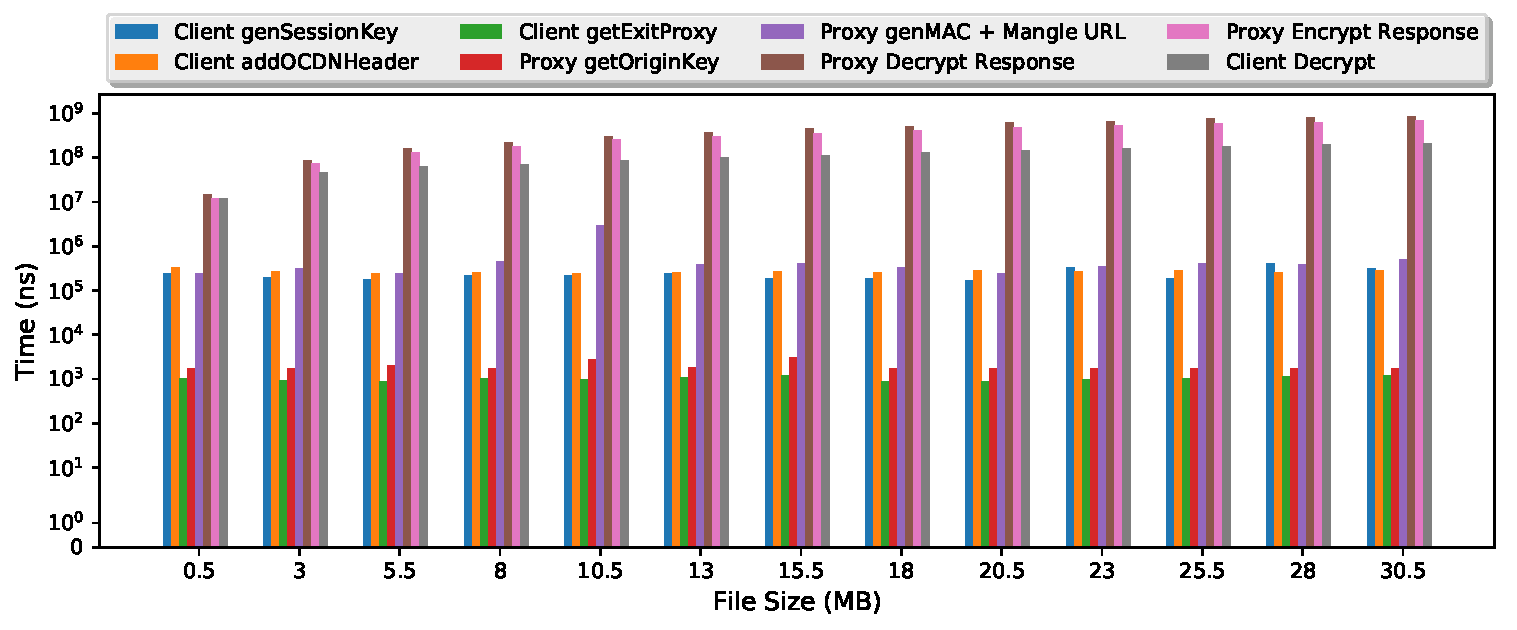
\includegraphics[width=.34\textwidth]{loggrouped}
%\caption{Overhead of different operations performed by \system{}.}
%\label{fig:overhead2}
%\end{figure}

\subsection{Scalability}
For evaluating performance, we are also concerned with how well \system{} will scale with more users 
and more URLs.  In particular, we need to reason about how much load is put on the exit proxies as the 
system grows; clients do not bare much load in the system as they simply proxy requests and the CDN is designed 
to handle high numbers of requests, therefore, we limit our scalability analysis to the exit proxies.  

As previously mentioned, we balance load among the proxies by using consistent hashing to assign URLs to 
exit proxies.  \system{} can additionally distribute load by replicating exit proxies, meaning that two exit proxies can 
have the same distributed hash table of shared keys.  This way, both exit proxies can accept requests from clients for 
the URLs they are responsible for.  Also worth noting is that the exit proxy is only recieving requests for the content 
corresponding to the shared keys it contains.  Therefore, as the number of clients grow, the exit proxy is still only responsible 
for its set of shared keys and subsequent URLs.  And as the number of URLs increase, the additional load per proxy is 
still low because of the load balancing properties of consistent hashing.  We also discuss in Section \ref{sec:discussion} how 
clients can set up exit proxies; this will further decrease the load per exit proxy because each exit proxy will be responsible 
for a smaller number of shared keys/URLs.